\documentclass[fleqn,twoside]{answers}
\usepackage{url}


% === dates ====
\RequirePackage{ifthen}
\let\oldtoday\today
\def\today{%
  \number\year-\ifcase\month\or%
  Jan\or Feb\or Mar\or Apr\or May\or Jun\or%
  Jul\or Aug\or Sep\or Oct\or Nov\or Dec\fi%
  -\ifthenelse{\number\day<10}{0}{}\number\day%
}

\begin{document}\pagestyle{empty}\thispagestyle{empty}
\setlength{\unitlength}{1in}%
\noindent\begin{picture}(0,0)
\put(0,-1.25){\begin{minipage}{\textwidth}
  \begin{center}
    \Large Answers to \\[1.5ex]
    \LARGE Theory of Computation \\[1.5ex]
    \Large Jim Hef{}feron \\[0.5ex]
    % \url{joshua.smcvt.edu/computation} \\[0.5ex]
    \large\href{https://hefferon.net/computation}{https://hefferon.net/computation}
  \end{center}
  \end{minipage}}
\put(0,-5.5){\begin{minipage}{\textwidth}
  \begin{center}
    % 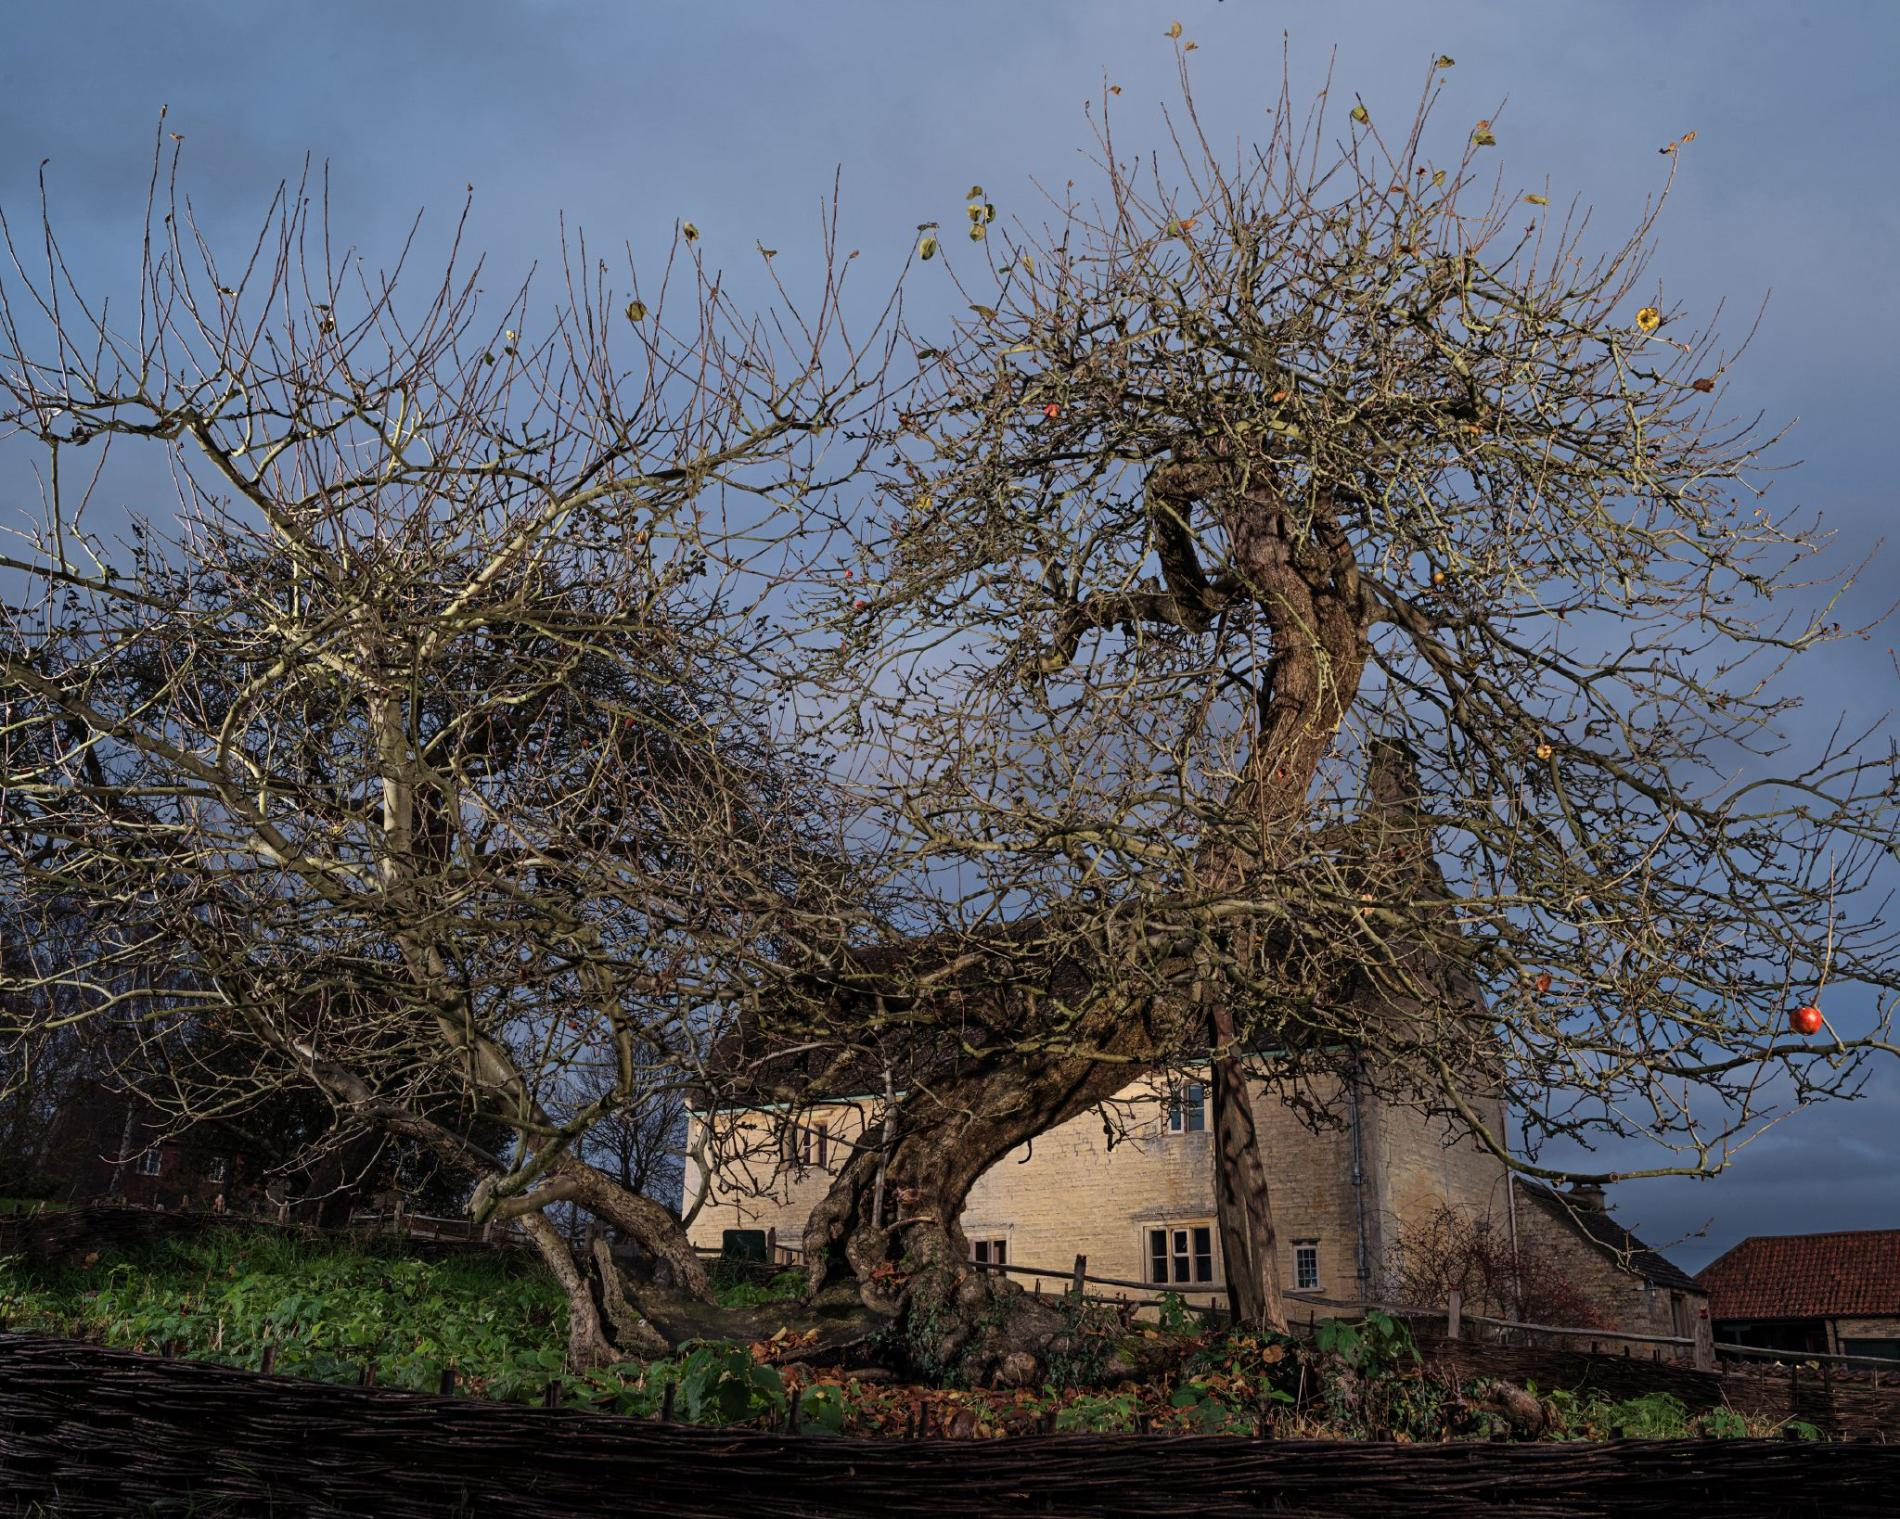
\includegraphics[width=\textwidth]{pix/newtonstree.jpg}
    
\includegraphics[width=0.6\textwidth]{automata/pix/flauros.jpg}
  \end{center}
  \end{minipage}}
\end{picture}
\clearpage
\vspace*{1in}
% \begin{center}
% \fbox{\parbox{0.95\textwidth}{
%   These answers are for the book version compiled \today.
%   If you find an error, I'd be very glad for a bug report. 
%   Please send to the contact information given at 
%   \href{https://hefferon.net}{\texttt{hefferon.net}}.
%   }}
% \end{center}
\par\noindent{\Large\bfseries About these answers}
\vspace{3ex}

% My friend William Zwicker from Union College describes what
% he calls the
% Clock Problem Problem.
% An example of a Clock Problem is:~between 4:38~pm on Tuesday and 5:15~am 
% Saturday, how many times will a clock's minute hand pass
% its hour hand?

% Bill saw a writeup of a complete solution to this class of problems.
% However, he observed, we don't ask this question for the answer.
% We ask it to give a challenging thinking problem to a bright student,
% in complete precision.
% That is, the point of some problems 
% is simply for students to do them.
 
A person who provides answers to 
text exercises has decisions:~some exercises or all?
or maybe all exercises to instructors only?
complete answers or summaries?
if summaries, what about proofs?.

The point of many of exercises is for students
to do them, and no doubt struggle with some.
Providing complete answers therefore has risks, including that
some students will just read the question and then read the answer and
so proceed with the sense that they understand, which is wrong.
But weighed against that is the worry that providing 
incomplete answers or hints,
or incomplete lists of answers such as odd only, 
can leave an honestly-trying person 
with no way to see what it is that they didn't see.

I have here provided complete answers, to all exercises.
My judgement is that my first attention is to
people honestly trying.
In particular, I expect that a good number of readers 
are working independently
and in the absence of an instructor the potential for help
is greater than the potential for harm.

In addition I find that doing the complete answers makes the questions better
because as I do them I am checking that the section contains all the needed
prerequisites for the answer,
that the question is clear, 
and I often go back to adjust or edit either the question or the section body.
Besides, I enjoy doing them, and there might as well be at least one 
person having a good time.

I am sometimes asked by instructors to provide a download of 
answers for some exercises, and to send out the rest 
only to instructors.
Putting aside the increased email burden for something that
I give away, and that I have no
way of knowing who is who, I'll say that
the askers have a different idea than I do of the relationship
between undergraduates and the Internet.
My experience has been that as with, say, 
a broad market Calculus text, any student will be
able within minutes to get the complete answer document. 


\begin{flushright}
  \begin{tabular}{l@{}}
    Jim Hef{}feron   \\
    University of Vermont  
  \end{tabular}
\end{flushright}


\vspace*{0pt plus 1fill}
\begin{flushright}
  \begin{minipage}{3in}
  \hspace{-1.5em}\textit{Cover:} Flauros, the sixty-fourth demon 
  and the Duke of Hell,
  who gives true answers of all things past, present, and future.
  Although, you should verify what he says for yourself.
  (Unless you can get him inside a triangle and then you're good, 
  although whether a triangle of roads, or rivers, or planets, is most unclear.)
  From \textit{Dictionnaire Infernal}, Jacques Albin Simon Collin de~Plancy, 
  1863. 
  \end{minipage} \\[2ex]
  \begin{minipage}{3in}
    \hspace{-1.5em}This PDF was compiled \today.
  \end{minipage}
\end{flushright}

\protect \chapter {Mechanical Computation}
\begin{ans}{1}
  Here is the trace.
\end{ans}
\begin{ans}{1}
It halts at the first step, because there is no instruction matching
the current state and what's being read on the tape, because there
is no instruction.
\end{ans}
\begin{ans}{1}
  Here is the trace.
\end{ans}
\begin{ans}{5}
\begin{exparts}
\item As with a program, a Turing Machine can implement an algorithm.
But an algorithm may be implemented by more than one Turing Machine.
For instance, we can do a shell sort of a list of five numbers
with two different Turing Machines, if only by renaming some of the states.
In the words of M~Davis \autocite{Davis16}, ``[Church's Thesis] says
nothing about what algorithms ARE.
It is about what algorithms can and can not DO.''
\textit{Comment:}~there is no widely agreed-upon definition of algorithm,
which is odd as algorithms are a central study in Computer Science.
\item A Turing Machine is a single-purpose device.
For instance, we may write a Turing Machine to multiply two of its inputs.
But today we use ``computer'' to mean a general-purpose, that is, programmable,
device.
\textit{Comment:} we will later see that there are general-purpose
Turing Machines, so the distinction is blurry, one of connotation rather
than of precise definition.
\end{exparts}
\end{ans}
\begin{ans}{5}
\begin{exparts}
\item The tape, as given in the definition, is not infinite.
It is unbounded.

For an analogy, consider the dictionary definition of a book.
In that definition there is no upper limit on the number of pages.
But no book, no actual bound collection of pages, has infiniteyl many.
So also, no halting Turing machine computation uses infinitely much tape
(the number of tape squares used is less than or equal to the number of
steps in the computation).

While it is true that you can easily write a Turing machine that does not
halt and that just keeps using more and more tape, at no step of the
calculation is the amount of tape infinite.
It never runs out\Dash it is unbounded\Dash but it is never infinite.

\item It is a model.
A model necessarily discards some aspects of the situation it models.
See \autocite{wiki:MapStory}.
(Besides, just to be argumentative for the sheer pleasure of it,
whether the universe is finite\Dash either just currently
finite, or finite into any unbounded future\Dash is not clear.
In any event it is not a mathematical question.)
\end{exparts}
\end{ans}
\begin{ans}{5}
(From \autocite{blass}.)
The first benefit that we get from this thesis is that it lets us
connect formal mathematical theorems to real-world issues of computability.
For example, the theorem that the word problem for groups is Turing-undecidable
has the real-world interpretation that no algorithm can solve all instance of
the word problem.

The second benefit is in mathematics itself, specifically in computability
theory.
Published proofs that something is Turing-computable almost never proceed by
exhibiting a Turing-machine program, or indeed a program in any actual
computing language.
Sometimes, if the matter is simple enough, they provide some sort of
pseudo-code.
Most often, though, they merely give an informal description of an algorithm.
It is left to the reader to see that this actually does give an algorithm
(in the intuitive sense) and therefore, by the Church-Turing thesis, could be
simulated by a Turing machine.
The usual situation is that, although experts in Turing-machine programming
would (if they existed) be able to routinely convert the intuitive algorithm
into a Turing machine program, the program would be too large and
complicated to be worth writing down.
\end{ans}
\begin{ans}{5}
Lance Fortnow says it perfectly,
``Computation is about process, about the transitions made from one state
of the machine to another. Computation is not about the input and the output,
point A and point B, but the journey. \ldots{}
You can feed a Turing machine an infinite digits of a real number
(Siegelmann), have computers interact with each other (Wegner-Goldin),
or have a computer that perform an infinite series of tasks (Denning) but
in all these cases the process remains the same, each step following
Turing's model.''
\autocite{Fortnow10}.
\end{ans}
\begin{ans}{3}
This is an implementation.
\begin{lstlistings}
(define (M x)
   (if (<= x 100)
       (M (M (+ x 11)))
       (- x 10)))
\end{lstlistings}
It outputs $91$ for all inputs $x\in\set{0, \ldots 101}$.
For larger inputs it outputs $x-10$.
\end{ans}
\begin{ans}{3}
The derivation for factorial is this.
\begin{equation*}
  \factorial(y)=\begin{cases}
              1                  &\text{if $y=0$}  \\
              \product(\factorial(z),\successor(z))) &\text{if $y=\successor(z)$}
            \end{cases}
\end{equation*}
Here $g$ is a function of no inputs~$g(\,)=1$ and
$h(a,b)=\product(a,\successor(b))$.
\end{ans}
\begin{ans}{3}
\begin{exparts}
\item The constant function that always returns zero
$\mathcal{C}_0(\vec{x})$
is included the definition of primitive
recursion, \cref{def:PrimitiveRecursive}, as $\zero(\vec{x})=0$.
The function that always returns~$1$ is then
$\mathcal{C}_1(\vec{x})=\succ(\mathcal{C}_0(\vec{x}))$,
the function that returns~$2$ is
$\mathcal{C}_2(\vec{x})=\succ(\succ(\mathcal{C}_0(\vec{x})))$, etc.

\item Since the parts of the right-hand side of
  $\max(\set{x,y})=y+(x\propersub y)$ are all primitive recursive,
  then the $\max$ function is also primitive recursive.
  Similarly for $\min(\set{x,y})=x+y\propersum\max(\set{x,y})$.

\item For any $x,y\in\N$ either $x-y\geq 0$ or $y-x\geq 0$.
Thus
$\operatorname{absdiff}(x,y)=\operatorname{propersub}(x,y)+\operatorname{propersub}(y,x)$ and since addition is primitive recursive,
$\operatorname{absdiff}(x,y)$ is therefore primitive recursive.

\item This primitive recursion defines $\operatorname{sign}$.
\begin{equation*}
  \operatorname{sign}(y)=
    \begin{cases}
      0   &\case{\text{if $y=0$}}  \\
      1   &\case{\text{if $y=\succ(z)$}}
    \end{cases}
\end{equation*}

\item A primitive recursion will do
\begin{equation*}
  \operatorname{negsign}(y)=
    \begin{cases}
      1   &\case{\text{if $y=0$}}  \\
      0   &\case{\text{if $y=\succ(z)$}}
    \end{cases}
\end{equation*}
but we can also observe that
$\operatorname{negsign}(y)=1-\operatorname{sign}(y)$, that is,
$\operatorname{negsign}(y)=\operatorname{propersub}(1,\operatorname{sign}(y))$.

\item The one is
$\operatorname{lessthan}(x,y)=\operatorname{sign}(\operatorname{propersub}(y,x))$
while the other is
$\operatorname{greaterthan}(x,y)=\operatorname{sign}(\operatorname{propersub}(x,y))$.

\item
We have $\operatorname{not}(x)=1-x=\operatorname{propersub}(1,x)$.
For the two-input ones,
$\operatorname{and}(x,y)=x\cdot y=\product(x,y)$
and
$\operatorname{or}(x,y)=\operatorname{sign}(x+y)$
(an alternative is $\operatorname{or}(x,y)=1-((1-x)\cdot (1-y))$).

\item
$\operatorname{equal}(x,y)=\operatorname{negsign}(\operatorname{lessthan}(x,y)+\operatorname{greaterthan}(x,y))$

\item
The first is
$m(x)=7\cdot\operatorname{equal}(x,1)
      +9\cdot\operatorname{equal}(x,5)$
(note the use of addition and multiplication, which were shown to be
primitive recursive in the subsection body).
The second is similar
$n(x,y)=7\cdot\operatorname{equal}(x,1)\cdot\operatorname{equal}(y,2)
        +9\cdot\operatorname{equal}(x,5)\cdot\operatorname{equal}(y,5)$.

\end{exparts}
\end{ans}
\begin{ans}{3}
\begin{exparts}
\item Since $g$ is given as primitive recursive,
this function is also primitive recursive
$h(a,b)=\plus(a,g(b))$ because it uses composition.
With that, this primitive recursion will do the bounded sum.
\begin{equation*}
  f(y)=
    \begin{cases}
      0          &\case{\text{if $y=0$}}  \\
      h(f(z),z)  &\case{\text{if $y=\succ(z)$}}
    \end{cases}
\end{equation*}

\item
This is similar to bounded sum.

\item
Consider the bounded product function.
\begin{equation*}
  P_p(\vec{x},m)=\prod_{0\leq i<m} p(\vec{x},i)
\end{equation*}
Note that (i)~if $P_p(\vec{x},m)=1$ then $P_p(\vec{x},i)=1$ for all $i<m$,
and (ii)~if $P_p(\vec{x},m)=0$ then $P_p(\vec{x},i)=0$ for all~$i\geq m$.

Next consider the bounded sum function.
\begin{equation*}
  S_{P_p}(\vec{x},m)=\sum_{0\leq i<m} P_p(\vec{x},m)
\end{equation*}
Because of (i) and~(ii), $S_{P_p}(\vec{x},m)$ is the least number~$i$ such that
$p(\vec{x},i)=0$, as desired.

Now just define $M(\vec{x},m)$ by cases.
\begin{equation*}
  M(\vec{x},m)=
  \begin{cases}
    m     &\case{\text{if $S_{P_p}(\vec{x},m)=0$}} \\
    S_{P_p}(\vec{x},m)  &\case{\text{otherwise}}
  \end{cases}
\end{equation*}

\item This is the idea.
\begin{equation*}
  U(\vec{x},m)=
  \begin{cases}
    1    &\case{\text{if $m=0$}}   \\
    p(\vec{x},m)\cdot U(\vec{x},z)  &\case{\text{if $m=\succ(z)$}}
  \end{cases}
\end{equation*}
To be formal we have to do some more work such as
expressing the multiplication
$p(\vec{x},m)\cdot U(\vec{x},z)$ as $\product(p(\vec{x},m), U(\vec{x},z))$.

\item Take $E(\vec{x},m)=1\dotminus \hat{E}(\vec{x},m)$, where the latter
function is below.
\begin{equation*}
  \hat{E}(\vec{x},m)=
  \begin{cases}
    0    &\case{\text{if $m=0$}}   \\
    (1\dotminus p(\vec{x},m))\cdot \hat{E}(\vec{x},z)
        &\case{\text{if $m=\succ(z)$}}
  \end{cases}
\end{equation*}

\item This follows straight from the definition on noting that one suitable
bound on the quotient~$k$ is the dividend~$y$, that is,
$\operatorname{divides}(x,y)=
\exists k\leq y[y=x\cdot k]$.

\item As in the prior item, we need only find a suitable bound.
Here, $\operatorname{prime}(y)=1$ if and only if
both $1<y$ and
there is no $x< y$ with $x>1$ and $\operatorname{divides}(x,y)$,
All of those components are primitive recursive.
\end{exparts}
\end{ans}
\begin{ans}{3}
\autocite{Davis}
Suppose that if two functions $\map{f,\hat{f}}{\N^{n+1}}{\N}$ both
satisfy \cref{def:PrimitiveRecursion}.
We will show that for all $\sequence{x_0,\ldots,x_{n-1},y}\in\N^{n+1}$
the two are equal $f(x_0,\ldots,x_{n-1},y)=\hat{f}(x_0,\ldots,x_{n-1},y)$,
by induction on~$y$.

For the base step,
they are equal when $y=0$ because they both equal $g(x_0,\ldots,x_{n-1})$.
For the inductive step,
suppose that they are equal for $y=0$, \ldots, $y=k$ and consider
the $y=k+1$ case.
\begin{align*}
  f(x_0,\ldots,x_{n-1},k+1)
  &=g(f(x_0,\ldots,x_{n-1},k),\,x_0,\ldots,x_{n-1},\,k)
  &=g(\hat{f}(x_0,\ldots,x_{n-1},k),\,x_0,\ldots,x_{n-1},\,k)
   =\hat{f}(x_0,\ldots,x_{n-1},k+1)
\end{align*}
The second equality follows from the induction hypothesis.
\end{ans}
\begin{ans}{3}
We have $\hyperoperation_4(2,2)=2^2=4$,
and $\hyperoperation_4(2,3)=2^{2^2}=2^4=16$.
The third is this.
\begin{equation*}
  \hyperoperation_4(2,4)=2^{2^{2^2}}=2^{16}=65536
\end{equation*}
\end{ans}

\end{document}